\section{Experiment: Bars and Framed Rectangles}

Visual cues can help converting graphical elements back to their real world variables. Cleveland and McGill introduced the bars and framed rectangles experiment which judges the elementary perceptual task of position along non-aligned scales~\cite{cleveland_mcgill}. 

\subsection{Hypotheses}

We proposed two hypotheses entering the elementary perceptual task experiment:

\begin{itemize}
	\item \textbf{H4.1} \textbf{Classifiers can leverage additional visual cues.} The original bar and framed rectangle experiment shows how visual cues aid humans in mapping graphical elements to quantitative variables. This should be the same for feed-forward neural networks since they are inspired by the visual system.
	\item \textbf{H4.2} \textbf{Weber's law can be transferred to computational perception.} Cleveland and McGill confirmed Weber's law based on the bar and framed rectangle experiment. For humans, the ability to perceive change within a distribution is proportional to the size of the initial distribution.
\end{itemize}

%\begin{figure}[t]
%	  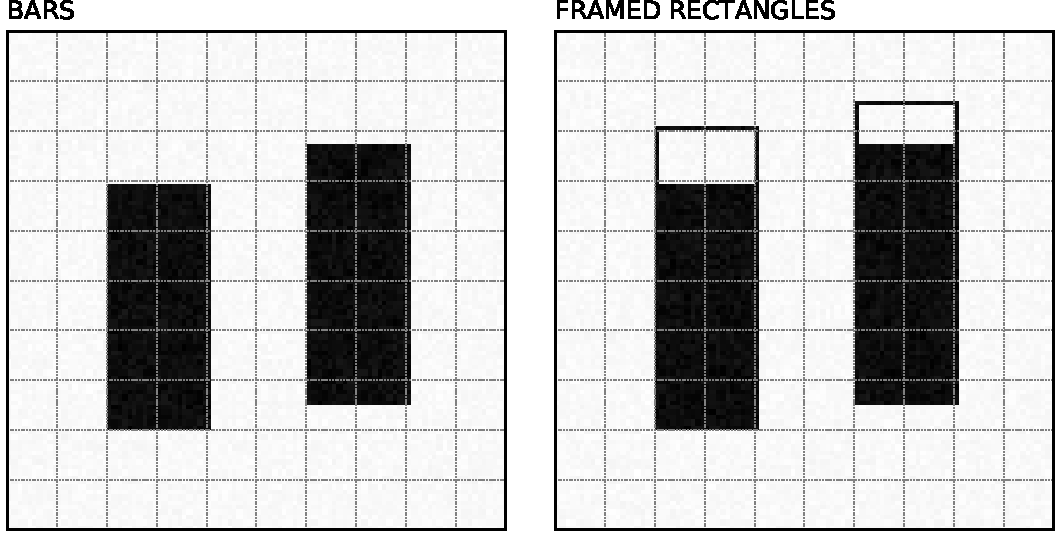
\includegraphics[width=\linewidth]{figure12_overview}
%  \caption{\textbf{Bars and Framed Rectangles Experiment.} Cleveland and McGill introduce the bars and framed rectangles experiment which measures the perceptual task of judging position along non-aligned scales. For humans, it is easier to decide which of two bars represent a larger height if a scale is introduced by adding framed rectangles (right). In this case, the right bar is heigher as visible with less free space when adding the frame. We evaluate whether such a visual aid also helps machines to perceive visually encoded quantities.}
%	\label{fig:bars_and_framed_rectangles_experiment}
%\end{figure}
%\begin{table}[h]
%\centering
%\caption{\textbf{Bars and Framed Rectangles Experiment.} Cleveland and McGill introduce the bars and framed rectangles experiment which measures the perceptual task of judging position along non-aligned scales. For humans, it is easier to decide which of two bars represent a larger height if a scale is introduced by adding framed rectangles. In this case, the right bar is heigher as visible with less free space when adding the frame. We evaluate whether such a visual aid also helps machines to perceive visually encoded quantities.}
%\resizebox{\linewidth}{!}{
%\begin{tabular}{lllr}
%	\toprule
%	\multicolumn{2}{l}{~} & ~ & Permutations\\
%
%	\midrule
%	\raisebox{-.85\height}{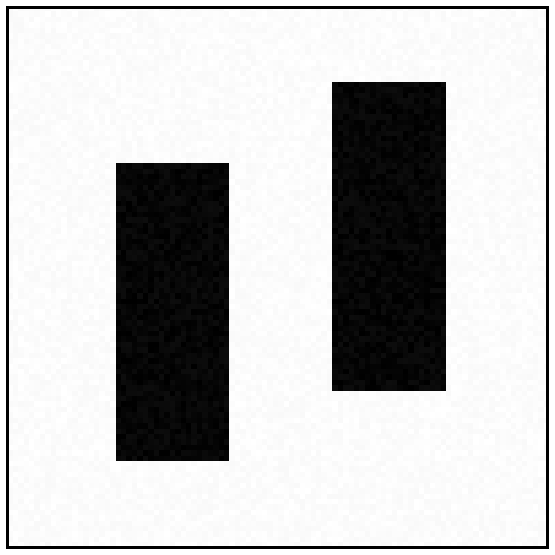
\includegraphics[width=.5in]{figure12_0.pdf}} & \makecell[tl]{\emph{Bars}\\~~~Perceptual Task: \emph{Length}\\~~~JND: $X\%$\\~ \\~~~~~~~~~~~~~~~~~~~~~~~~~~~~~~~~ \\} &~& \makecell[tr]{~\\ $57,600$}\\
%
%
%	\midrule
%	\raisebox{-.85\height}{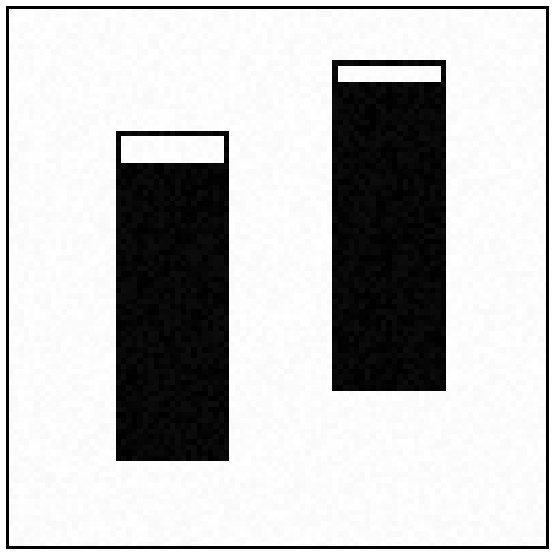
\includegraphics[width=.5in]{figure12_1.pdf}} & \makecell[tl]{\emph{Framed Rectangles}\\~~~Perceptual Task: \emph{Position}\\~~~JND: $X\%$\\~ \\~~~~~~~~~~~~~~~~~~~~~~~~~~~~~~ \\} &~& \makecell[tr]{~\\ $57,600$}\\
%
%
%	\bottomrule
%\end{tabular}
%}
%\label{tab:bars_and_framed_rectangles_parameters}
%\end{table}


\subsection{Weber-Fechner's Law}

As identified by Cleveland and McGill, the bar and framed rectangle experiment is closely related to Weber's law. This psychophysics law states that perceivable difference within a distribution is proportional to the initial size of the distribution. Weber's law goes hand-in-hand with Fechner's law. We conduct an additional experiment based on the original illustrations of the Weber-Fechner law to investigate whether this law can be applied to computational perception of our classifiers (Fig.~\ref{tab:weber_law}).

%\begin{figure}[t]
%	  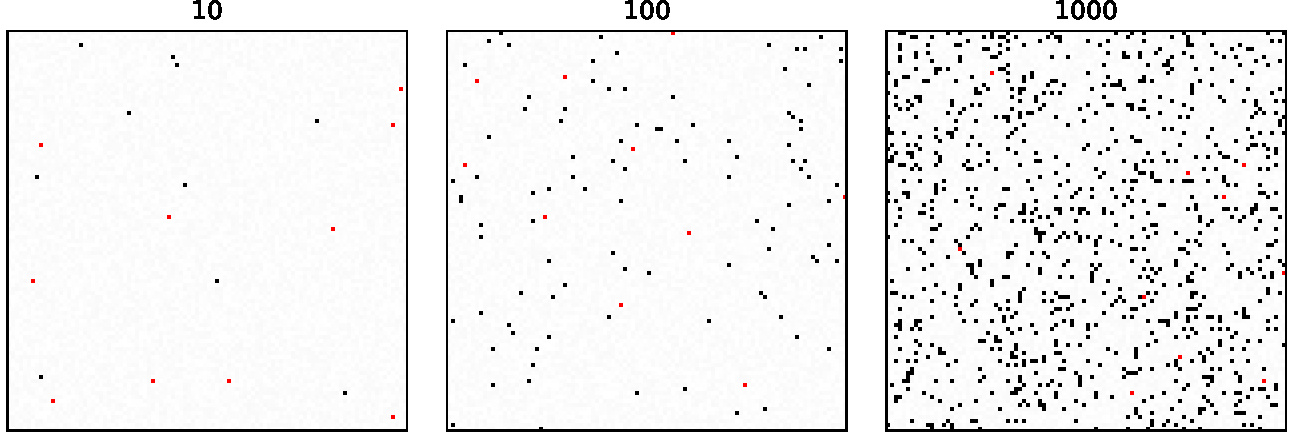
\includegraphics[width=\linewidth]{weber_overview}
%  \caption{\textbf{Weber-Fechner Law.} The Weber-Fechner law states that the perceivable differences within a distribution is proportional to the initial size of the distribution. The lower square contains 10 more dots than the upper one on both sides. However, the difference is easily perceivable on the left while the squares on the right almost look the same. We generate rasterized visualizations similar to this setup and evaluate our classifiers.}
%	\label{fig:webers_law}
%\end{figure}
%\begin{table}[h]
%\centering
%\caption{\textbf{Weber-Fechner Law.} The Weber-Fechner law states that the perceivable differences within a distribution is proportional to the initial size of the distribution. We create three different types of images initialized with 10, 100, and 1000 dots. We then mark randomly up to 10  dots in previously free pixels (here visualized in red). For humans, the difference is easily perceivable when the initial dot count is 10 but is hard when it is higher. We evaluate our classifiers on these rasterized visualizations.}
%\resizebox{\linewidth}{!}{
%\begin{tabular}{lllr}
%	\toprule
%	\multicolumn{2}{l}{~} & ~ & Permutations\\
%
%	\midrule
%	\raisebox{-.85\height}{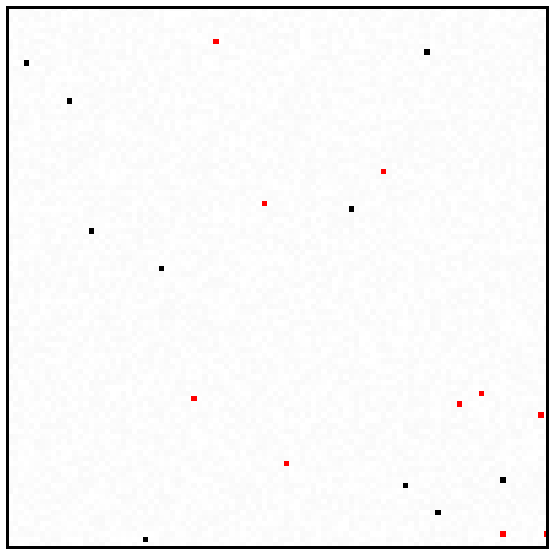
\includegraphics[width=.5in]{weber_0.pdf}} & \makecell[tl]{\emph{Base 10}\\~~~JND: $X\%$\\~ \\ ~~~~~~~~~~~~~~~~~~~~~~~~~~~~~~~~~~~~~~~~ \\} &~& \makecell[tr]{~\\ $10,000$}\\
%
%
%	\midrule
%	\raisebox{-.85\height}{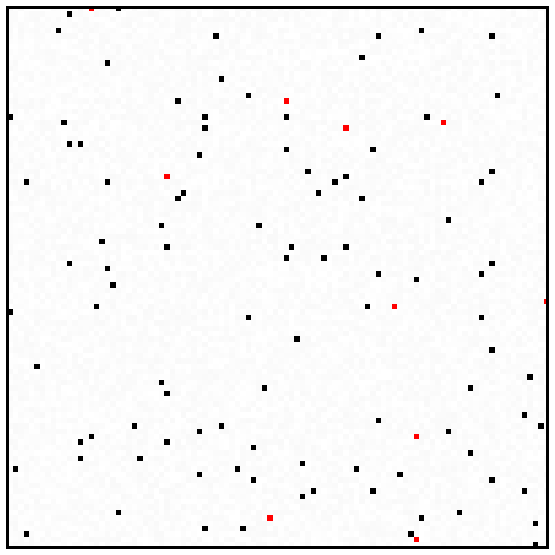
\includegraphics[width=.5in]{weber_1.pdf}} & \makecell[tl]{\emph{Base 100}\\~~~JND: $X\%$\\~ \\ ~~~~~~~~~~~~~~~~~~~~~~~~~~~~~~~~~~~~~~~~ \\} &~& \makecell[tr]{~\\ $10,000$}\\
%	
%	\midrule
%	\raisebox{-.85\height}{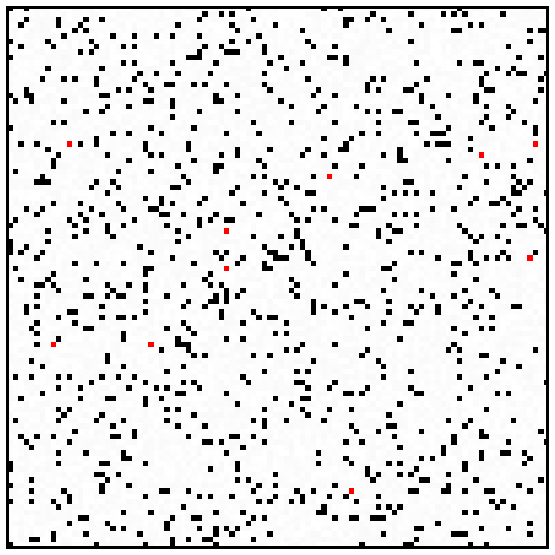
\includegraphics[width=.5in]{weber_2.pdf}} & \makecell[tl]{\emph{Base 1000}\\~~~JND: $X\%$\\~ \\ ~~~~~~~~~~~~~~~~~~~~~~~~~~~~~~~~~~~~~~~~ \\} &~& \makecell[tr]{~\\ $10,000$}\\
%
%	\bottomrule
%\end{tabular}
%}
%\label{tab:weber_law}
%\end{table}


\subsection{Results}

First run indicates that framed rectangles perform better but we dont really know it yet.

\begin{figure}[t]
	  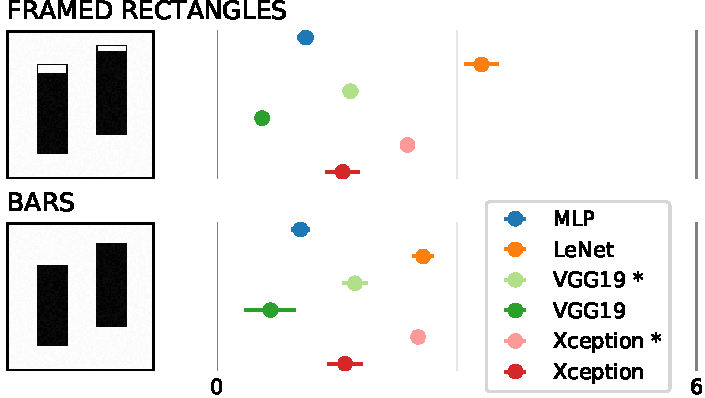
\includegraphics[width=\linewidth]{figure12_mlae_better_all.pdf}
  \caption{\textbf{Computational results of the Bars-and-Framed-Rectangles experiment.} Log absolute error means and 95\% confidence intervals for the \emph{bars-and-framed-rectangles experiment} as described by Cleveland and McGill~\cite{cleveland_mcgill}. We test the performance of a Multi-layer Perceptron (MLP), the LeNet Convolutional Neural Network, as well as feature generation using the VGG19 and Xception networks trained on ImageNet.}
	\label{fig:figure12_mlae}
\end{figure}

\begin{figure}[t]
	  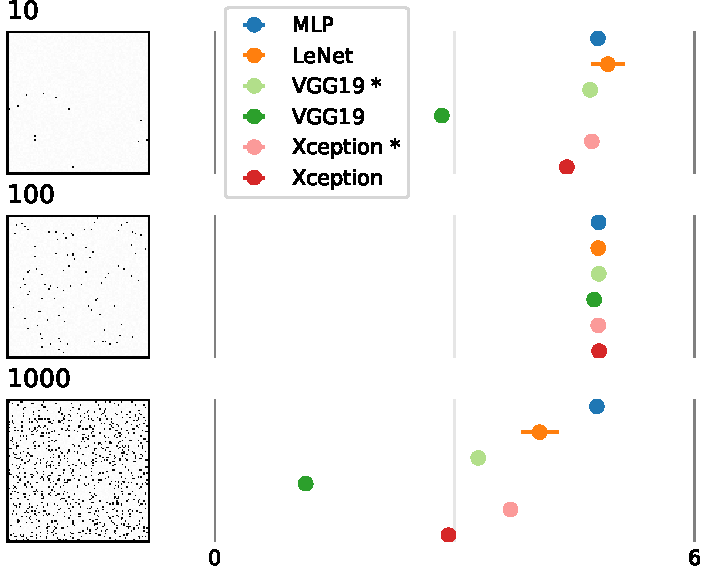
\includegraphics[width=\linewidth]{weber_mlae_noise_all.pdf}
  \caption{\textbf{Computational results of the Weber-Fechner's Law experiment.} Log absolute error means and 95\% confidence intervals for the \emph{bars-and-framed-rectangles experiment} as described by Cleveland and McGill~\cite{cleveland_mcgill}. We test the performance of a Multi-layer Perceptron (MLP), the LeNet Convolutional Neural Network, as well as feature generation using the VGG19 and Xception networks trained on ImageNet.}
	\label{fig:weber_law}
\end{figure}
